\chapter{Implementation}\label{ch:implementation}

\section{Setting up the workspace}\label{sec:setting-up-the-workspace}

\subsection{Creating a GitHub repository}\label{subsec:creating-a-git-repository}

\begin{figure}[H]
    \centering
    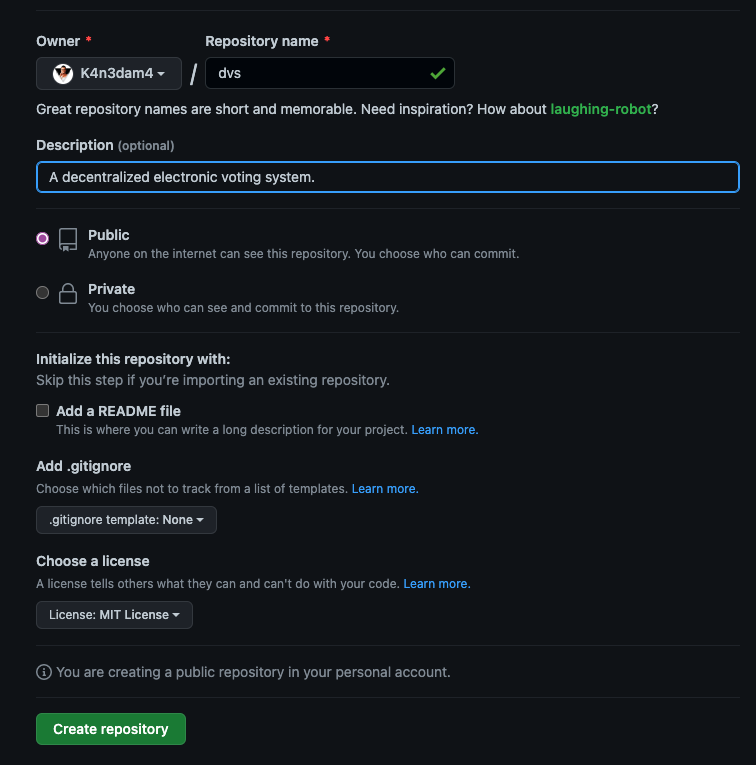
\includegraphics[scale=0.4]{initializing-repository}
    \caption{Creating a Github repository}
    \label{fig:initializing-repository}
\end{figure}

For the reasons discussed in~\cref{subsec:versioning}, the first step in the development process was the creation of a GitHub repository.
As seen in~\cref{fig:initializing-repository}, we changed the license from \emph{None} to \emph{MIT License}.
At the same time, the repository itself was initialized containing neither a README nor a .gitignore file, as these are automatically created by nx (see~\cref{subsec:creating-a-monorepo-using-nx}).

\subsection{Creating a monorepo using nx}\label{subsec:creating-a-monorepo-using-nx}

Creating a monorepo with nx is a straightforward process using the nx-provided executable package \emph{create-nx-workspace} with \gls{npx}.

\begin{figure}
    \begin{subfigure}[b]{\textwidth}
        \centering
        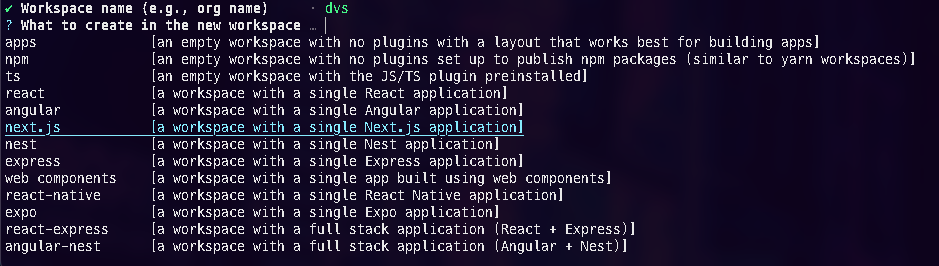
\includegraphics[width=\textwidth]{nx-workspace-options-0}
        \caption{Options for app templates nx can automatically build during initialization}
        \label{fig:nx-workspace-options-0}
    \end{subfigure}
    \begin{subfigure}[b]{0.5\textwidth}
        \centering
        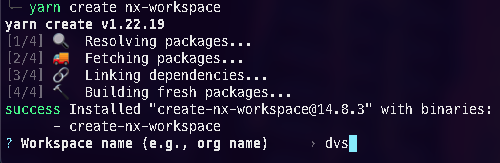
\includegraphics[width=\textwidth, height=85px]{nx-workspace-name}
        \caption{Naming the workspace}
        \label{fig:nx-workspace-name}
    \end{subfigure}
    \begin{subfigure}[b]{0.5\textwidth}
        \centering
        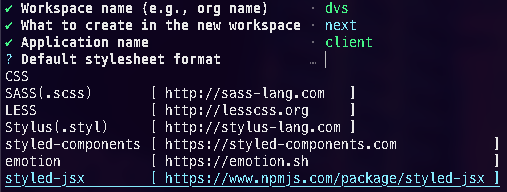
\includegraphics[width=\textwidth]{nx-workspace-options-1}
        \caption{Default style format options}
        \label{fig:nx-workspace-options-1}
    \end{subfigure}
    \caption{Setting up a nx workspace}
    \label{fig:setting-up-nx-workspace}
\end{figure}

After initiating the process by typing \mintinline{text}{yarn create nx-workspace} in the terminal, nx allows developers to name (see~\cref{fig:nx-workspace-name}) the project.
Next, developers are offered several template options for an initial application nx then automatically adds to the workspace (see~\cref{fig:nx-workspace-options-0,fig:nx-workspace-options-1}).
Given these options, we initialized the workspace with a Next.js application for the client side of the voting system.
Alternatively, we could have initialized it with Nest.js, but the order in which client and server applications were added to the workspace was irrelevant in this context.

\section{Setting up the backend}\label{sec:setting-up-a-nest.js-backend}

\subsection{Creating a Nest.js application}\label{subsec:creating-a-nest.js-application}

The installation of a plugin with \mintinline[breaklines]{text}{yarn add -D @nrwl/nest} was necessary to let nx handle the installation process of the Nest.js application.
After installing the plugin, we added a new Nest.js application to the workspace using the \mintinline[breaklines]{text}{nx g @nrwl/nest:app api} command, where \emph{api} is the name given to the application.

To maintain scalability, we combined Nest.js's modular design with nx's \emph{libs} directories, meaning backend controllers and services were split up and installed into \emph{libs/api} rather than the application directory.
As mentioned in~\cref{subsec:nx}, modularizing code within the \emph{libs} directory makes it reusable in all workspace applications sharing the same scope.
Hence, all future applications that might be added to the project will also be able to access that code if needed, thus making it easier to adhere to \gls{DRY} principles.

\subsection{Creating a PostgreSQL database}\label{subsec:creating-a-postgresql-database}

To handle database entries, we created a new Nest.js module, \emph{prisma}, in the \emph{libs/api} folder.
Then, we installed Prisma as a devDependency with \mintinline[breaklines]{text}{yarn add -D prisma}, which provided basic tooling for databases, such as creating type-safe schemas, a built-in migration system, and a \gls{GUI} to display and edit database entries.
Following the installation process, we created a docker-compose.yml, enabling the application to run dockerized PostgreSQL databases during development, test, or production builds (see listing~\ref{lst:docker-compose.yml}).

\codeFromFile{yaml}{code_snippets/docker-compose.yml}{Docker-compose.yml used in the prisma module}{Docker-compose.yml used in the prisma module}{lst:docker-compose.yml}

Having created a docker-compose file, along with the commands in the prisma module’s project.json and the project’s package.json necessary to run the database, we added a core Nest.js module (see listing~\ref{lst:core-module}) that makes configurations like the database \gls{URL} available throughout the Nest.js application.
Consequently, we could connect the Nest.js application to the database through the prisma service (see listing~\ref{lst:prisma-service}) using the \gls{URL} from the core module.

\codeFromFile{ts}{code_snippets/nest-core-module.ts}{Core module}{Core module}{lst:core-module}
\codeFromFile{ts}{code_snippets/nest-prisma-service.ts}{Prisma service}{Prisma service}{lst:prisma-service}

\section{Smart Contracts}\label{sec:smart-contracts}
















